% Source: https://tex.stackexchange.com/a/688469/6880

\documentclass[tikz,border=1.618]{standalone}

\tikzset{
  colour/.style = {
    circle,
    draw,
    fill=white,
    font=\small,
    inner sep=0.2pt,
    midway% <-- added
  },
  pics/cap/.style = {
    code = {
      \node[vertex](0) at (0,0){};
      \foreach \x in {#1} {
         \pgfmathtruncatemacro\y{\x-1}
         \node[vertex](\x) at (\x,0){};
         \draw(\y) to [out=60, in=120] node[colour]{$\x$} (\x);
      }
    }
  },
  vertex/.style = {
    circle,
    radius=1mm,
    inner sep=-2.0pt,
    fill=black
  },
}

\begin{document}
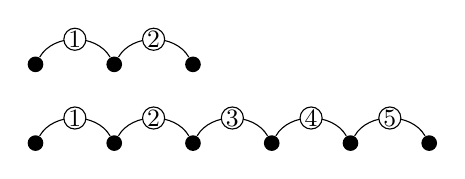
\begin{tikzpicture}
  \pic at (0, 0) {cap={1,2}};
  \pic at (0,-1) {cap={1,...,5}};
\end{tikzpicture}
\end{document} 
